\chapter{Theoretical Background}
\label{chap:theoretical-background}

This chapter introduces the Tsetlin Machine, a method for pattern recognition based on propositional logic and game theory. We briefly examine the ideas developed in the original research~\cite{granmo2021tsetlinmachinegame, glimsdal2021coalescedmultioutputtsetlinmachines} that were necessary for our work, explaining how the model is designed from the ground up. Finally, we discuss scenarios where this approach has the potential to be a viable alternative to neural networks. For a more extensive introduction to Tsetlin Machines, refer to~\cite{granmo2022tsetlinmachinebookchap1, granmo2022tsetlinmachinebookchap2}.

\section{Tsetlin Machine Overview}
The emergence of the TM is rooted in the development of a lesser-known, yet fundamental and versatile learning mechanism called the Tsetlin Automaton, developed by M.L. Tsetlin in the early 1960s~\cite{granmo2021tsetlinmachinegame, tsetlin1961behaviour}. Further research on this topic proposes a novel technique for complex large scale classification constructed using Tsetlin Automata~\cite{granmo2021tsetlinmachinegame}.

\paragraph{Pattern recognition}
The most important distinction of the TM lies in how it addresses pattern recognition problems. While the accuracy of a machine learning technique is related to its capability to represent patterns, the TM decomposes complex problems into self-contained sub-patterns~\cite{granmo2021tsetlinmachinegame}. Instead of using the complex arithmetic found in neural networks, this method utilizes Boolean algebra, which is the basis of how digital computers operate. As a result, the machine captures the structure of the data by expressing patterns as conjunctive clauses in propositional logic.

\paragraph{Logic-based approach}
The TM processes input features as bits to construct propositional logic expressed as ``If-Then'' rules, which offers both computational simplicity and interpretability. In short, given an input vector of propositional variables $X = (x_1, \dots, x_n) \in \{0,1\}^n$, we add their negated counterparts $\overline{x}_k = 1 - x_k$ to build a set of literals $L = \{l_1 \dots, l_{2n}\}$. From these literals, we construct conjunctive clauses that determine the output vector $Y = (y_1, \dots, y_m) \in \{0,1\}^m$. For example, clause $C(X) = x_1 \land x_2 = x_1 x_2$ consists of literals $\{x_1, x_2\}$ and outputs $1$ if and only if $x_1 = x_2 = 1$~\cite{granmo2021tsetlinmachinegame}. The simple inference structure of the TM can be seen in Figure \ref{fig:tsetlinmachinestructure}.

\begin{figure}[!htbp]
    \centering
    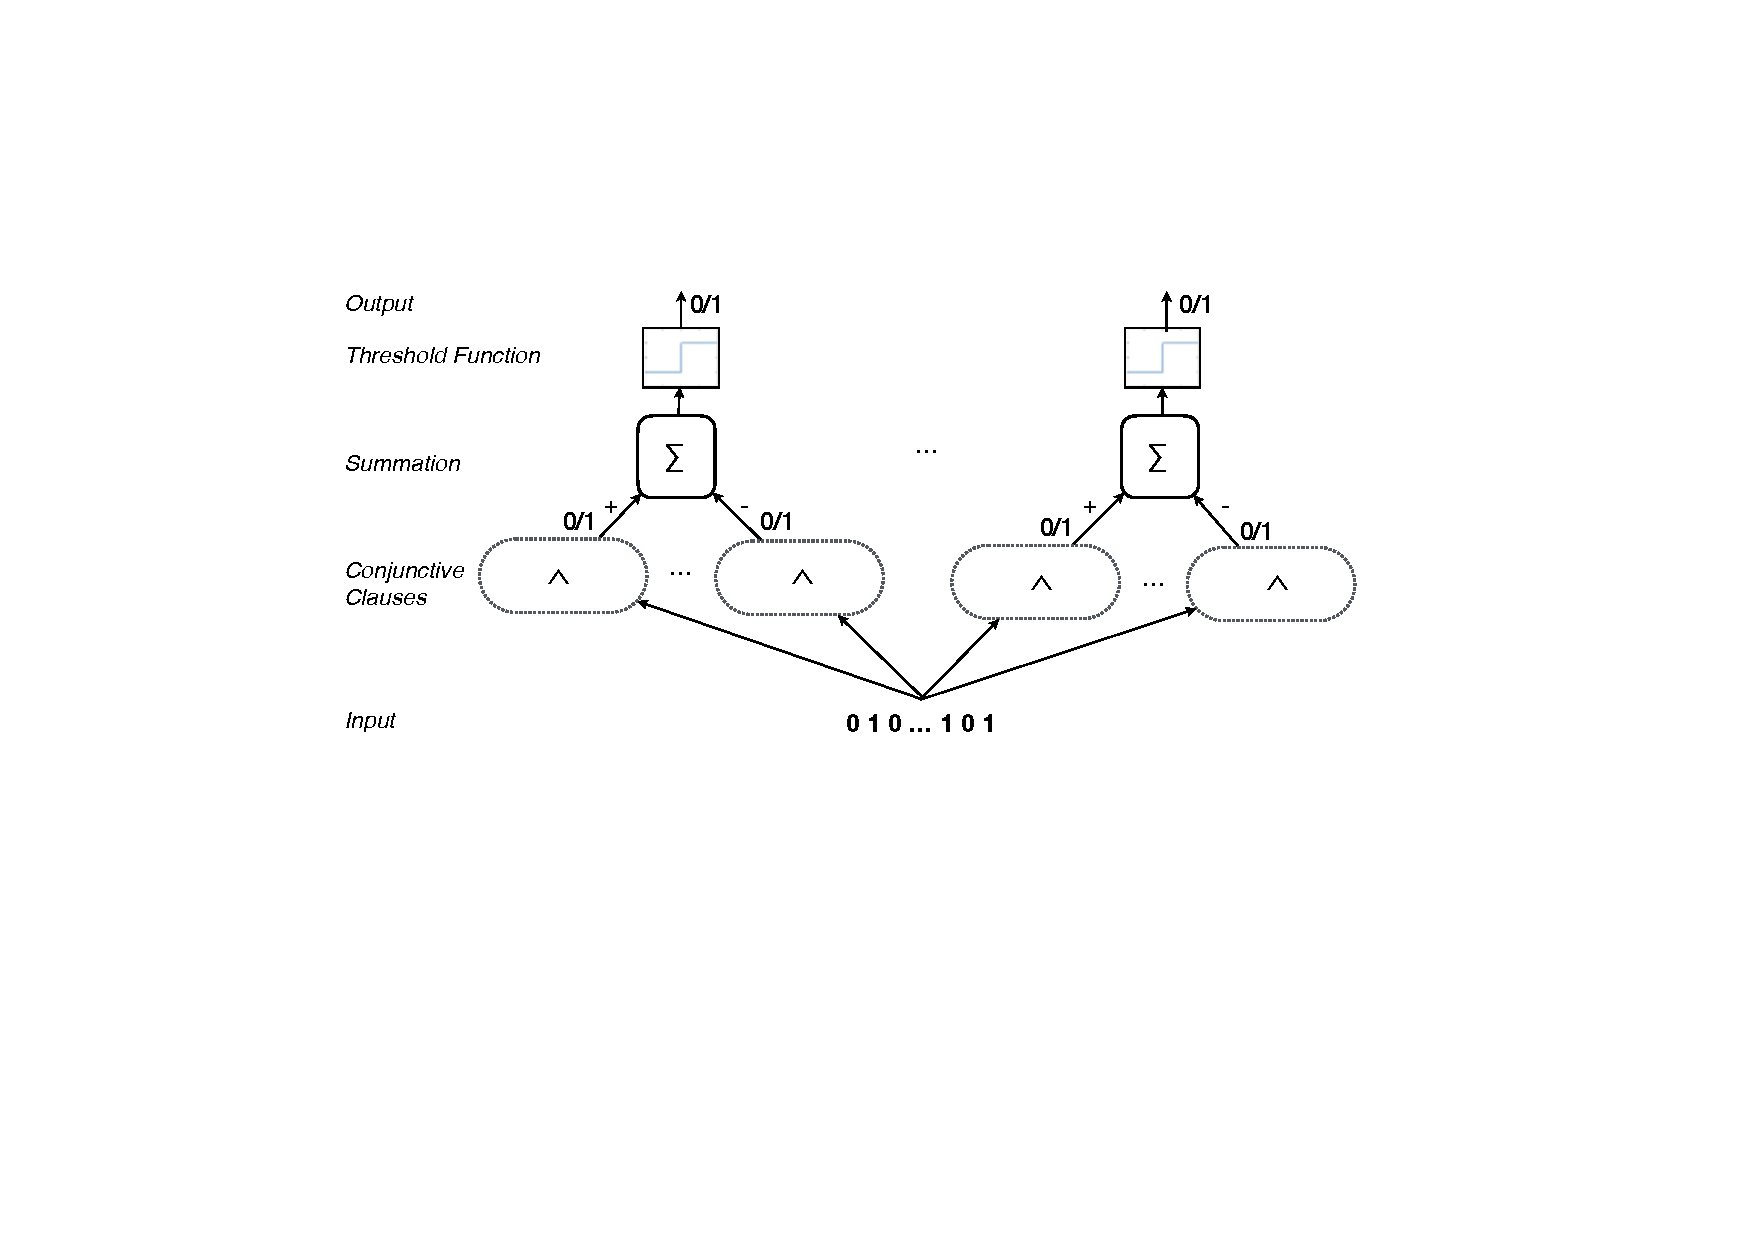
\includegraphics[width=.9\textwidth]{img/Overall_Architecture_Summation[1804.01508v15].pdf}
    \caption[The TM inference structure]{The TM inference structure (source: \cite{granmo2021tsetlinmachinegame})}
    \label{fig:tsetlinmachinestructure}
\end{figure}
\FloatBarrier

\section{Tsetlin Automaton}
The basic building block of a TM is the Tsetlin Automaton (Figure \ref{fig:tsetlinautomatongeneric}), recognized as one of the first solutions to the multi-armed bandit problem~\cite{granmo2021tsetlinmachinegame}. It is capable of learning the optimal action when operating in unknown stochastic environments and is considered the first Learning Automaton~\cite{narendra2012learning}.

\paragraph{Decision making}
The Tsetlin Automaton performs actions $\alpha_z, z \in \{1, 2\}$ sequentially in an environment. Each action $\alpha_z$ triggers a reward or a penalty. The action is rewarded with probability $p_z$, otherwise it is penalized. The reward probabilities are unknown to the automaton and may change over time. Under these conditions, the goal is to identify the action with the highest probability of reward using as few attempts as possible~\cite{granmo2021tsetlinmachinegame}.

\paragraph{State-based memory}
The Tsetlin Automaton operates as a finite-state machine with $2N$ states, as illustrated in Figure \ref{fig:tsetlinautomatongeneric}. The current state determines the action: action $\alpha_1$ is performed in states $1$ to $N$, while action $\alpha_2$ is performed in states $N+1$ to $2N$. State transitions control how the automaton learns. One set of state transitions is activated upon receiving a reward (solid lines in the figure), and another set of state transitions is activated upon receiving a penalty (dotted lines in the figure). This mechanism is designed to reinforce successful (reward producing) actions~\cite{granmo2021tsetlinmachinegame}.

\begin{figure}[!htbp]
    \centering
    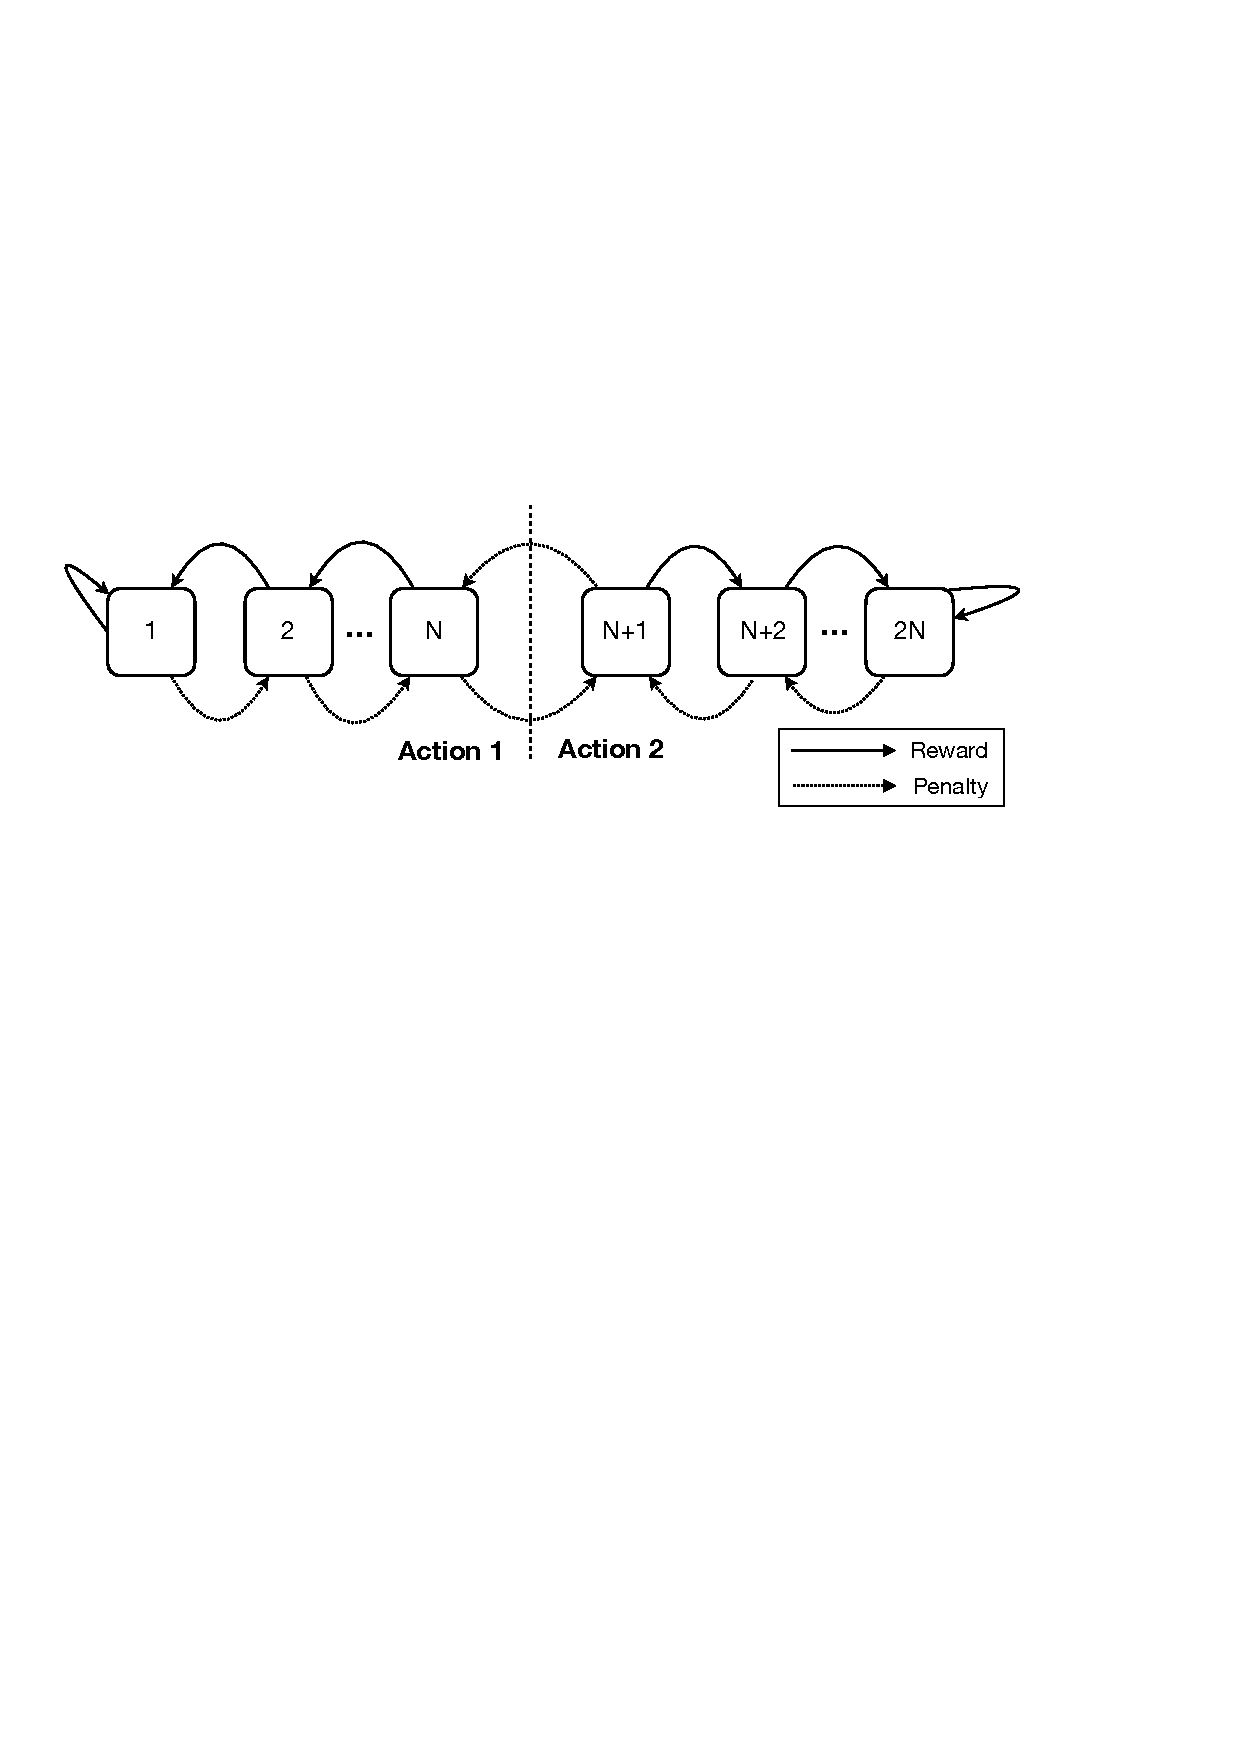
\includegraphics[width=.9\textwidth]{img/Tsetlin_Automaton_Generic[1804.01508v15].pdf}
    \caption[A Tsetlin Automaton for two-action environment]{A Tsetlin Automaton for two-action environment (source: \cite{granmo2021tsetlinmachinegame})}
    \label{fig:tsetlinautomatongeneric}
\end{figure}
\FloatBarrier

\section{Architecture and Problem Representation}
With the Tsetlin Automaton introduced as the main learning mechanism, the TM architecture arranges these automata into teams responsible for composing clauses. These teams collaborate to solve complex problems by optimizing pattern recognition accuracy. The generated clauses function as rules that vote for or against a specific class output while providing transparent logic to reach a final decision~\cite{granmo2021tsetlinmachinegame}. However, this approach requires specific input, where the data must be processed to produce features compatible with logic-based reasoning.

\paragraph{Binarization of data}
Since the TM operates using propositional logic, the input data is required to be represented as Boolean features. Nevertheless, this constraint can be mitigated with a simple pre-processing step that transforms the input into a suitable binary format. For categorical data, the universal one-hot encoding approach will suffice. For example, in the digit recognition problem with $8 \times 8$ images ($64$ elements) and $16$ possible brightness levels, the sample can be flattened and expanded to a binary vector. The handling of continuous features presents a different challenge, commonly addressed by segmenting data into predefined intervals. A continuous variable, such as temperature, can be transformed into a set of Boolean ranges like $[15^\circ,20^\circ)$ or $[20^\circ,25^\circ)$, allowing the machine to simply match the value.

\paragraph{Rule construction}
The mechanism for building a TM involves organizing Tsetlin Automata into teams, where each team is responsible for constructing a single conjunctive clause (AND-rule). These rules follow a logical pattern:
$$\textbf{if} \ \textit{condition} \ \textbf{then} \ \textit{class} \text{.}$$
For every potential literal in the input set (both original features and their negations), an assigned automaton determines whether to ``Include'' or ``Exclude'' that literal based on its internal state~\cite{granmo2021tsetlinmachinegame}. By combining these decisions through the AND-operator, the team produces a logical rule. For the vehicle classification task described in~\cite{granmo2022tsetlinmachinebookchap1}, a resulting rule can be expressed as: 
$$\textbf{if} \ \textit{Four Wheels} \ \textbf{and} \ \textit{Transports People} \ \textbf{then} \ \textit{Car} \text{.}$$

\paragraph{Class prediction by voting}
The TM, as shown in Figure \ref{fig:tsetlinmachinestructure}, feeds an input vector $X = (x_1, \dots, x_n) \in \{0,1\}^n$ to several conjunctive clauses for evaluation. The number of clauses used is a user-defined parameter $N$. The clauses are assigned into two groups based on polarity: positive clauses ($C_j^1, \ j \in \{1,\dots,N/2\}$) vote in favor of the target class ($y=1$), negative clauses ($C_j^0, \ j \in \{1,\dots,N/2\}$) vote against it ($y=0$)~\cite{granmo2021tsetlinmachinegame}.

While a standard clause learns to capture sub-patterns in $X$ and outputs the conjunction of its literals, the TM uses a specific mechanism for empty clauses ($L_j = \emptyset$). These clauses without literals are not required for classification and can be pruned from the inference structure, but during learning, they remain active:
$$C_j(X) = \begin{cases}
1, & \textbf{if } L_j=\emptyset \text{ during learning},\\
0, & \textbf{if } L_j=\emptyset \text{ during classification},\\
\bigwedge_{l_k \in L_j}l_k, & \textbf{if } L_j\neq\emptyset \text{.}
\end{cases}$$
The final classification $\hat{y}$ is reached through a majority vote. The clause evaluations are combined into a final output through summation and unit step thresholding:
$$\hat{y} = u \left( \sum_{j=1}^{N/2}C_j^1(X) - \sum_{j=1}^{N/2}C_j^0(X) \right)$$
where $u(v) = 1 \textbf{ if } v \ge 0 \textbf{ else } 0$. The summation allows the model to weigh positive against negative evidence found in the input $X$. The example classifier that captures the XOR-relation can be represented as $\hat{y} = u(x_1\overline{x}_2 + \overline{x}_1x_2 - x_1x_2 - \overline{x}_1\overline{x}_2)$~\cite{granmo2021tsetlinmachinegame}.

Figure \ref{fig:tsetlinmachineconfiguration} illustrates the TM configuration featuring two clauses: one with positive polarity and one with negative polarity. These clauses are determined by Tsetlin Automata, which select the literals to include from the set $L = \{x_1,x_2,\overline{x}_1,\overline{x}_2\}$. In this example, the positive clause results in the form $x_1\overline{x}_2$, while the negative clause forms $x_1x_2$.

\begin{figure}[!htbp]
    \centering
    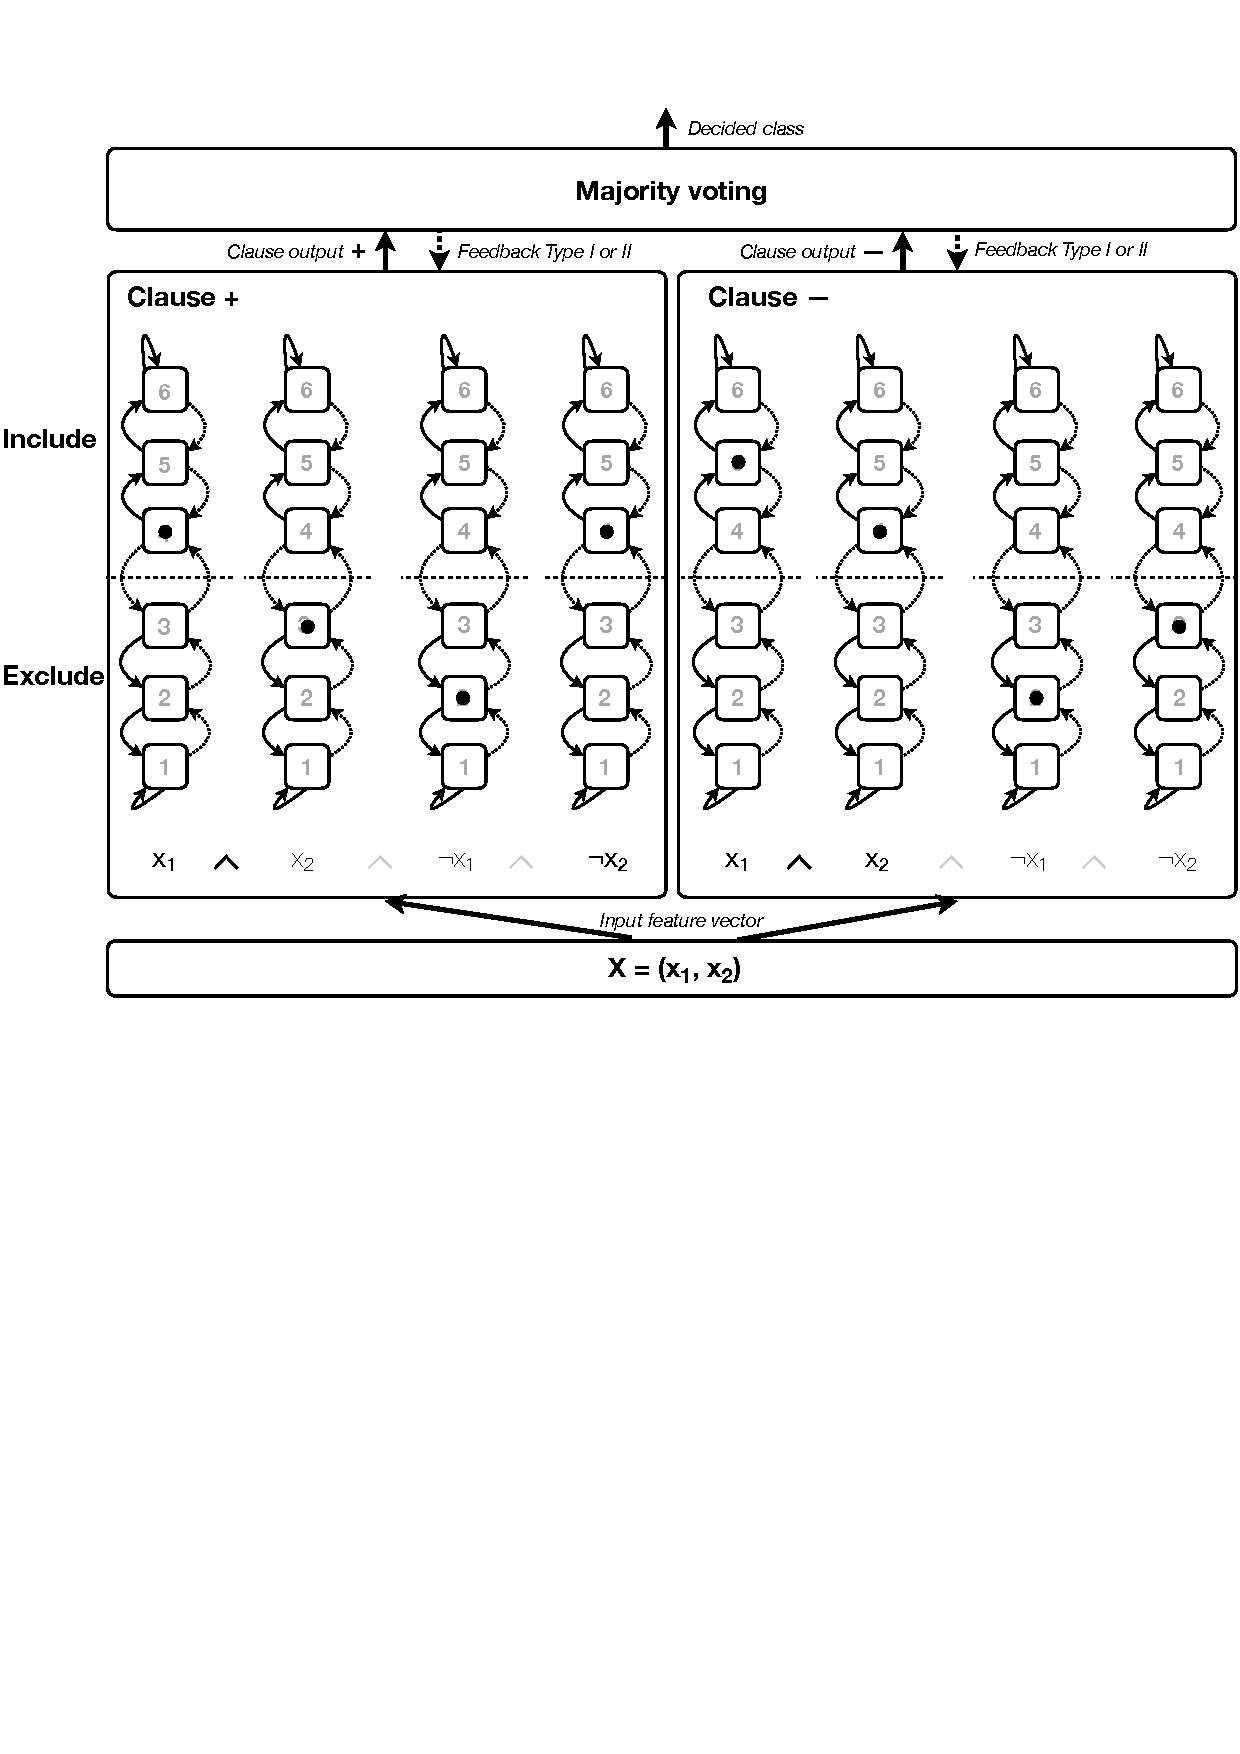
\includegraphics[width=.9\textwidth]{img/Tsetlin_Machine_Example_Configuration_Full[1804.01508v15].pdf}
    \caption[Two Tsetlin Automata teams]{Two Tsetlin Automata teams, each producing a conjunctive clause (source: \cite{granmo2021tsetlinmachinegame})}
    \label{fig:tsetlinmachineconfiguration}
\end{figure}
\FloatBarrier

\section{Learning Algorithm}
The learning mechanism of the TM functions through a game-theoretic approach, orchestrating Tsetlin Automata to maximize pattern recognition accuracy~\cite{granmo2021tsetlinmachinegame}. We follow the example found in~\cite{glimsdal2021coalescedmultioutputtsetlinmachines} to demonstrate this process.

\paragraph{IMDb review sentiment example}
To demonstrate the learning process, we consider the task of classifying the sentiment of movie reviews from the IMDb dataset. This problem uses a Set of Words (SoW) representation, where every word in the vocabulary acts as an input feature. Consider the review ``The movie was good, and I had popcorn.''. This text is converted into a binary input vector $X$. The inputs for words present in the review (e.g. ``good'' and ``movie'') are set to True, while the inputs for any missing words are set to False.

\paragraph{Memory}
Consider the clause designed to detect positive sentiment targeting the pattern ``good'' AND ``movie''. To manage this rule, the machine uses a team of Tsetlin Automata, assigning one automaton to track each potential literal. Figure \ref{fig:memoryimdb} illustrates the memory states maintained by this team. Feedback from the learning process increases these states to remember the literal longer when a reinforcing truth value is observed, and without such observations, the values decrease, causing the clause to eventually forget the literal.

\begin{figure}[!htbp]
    \centering
    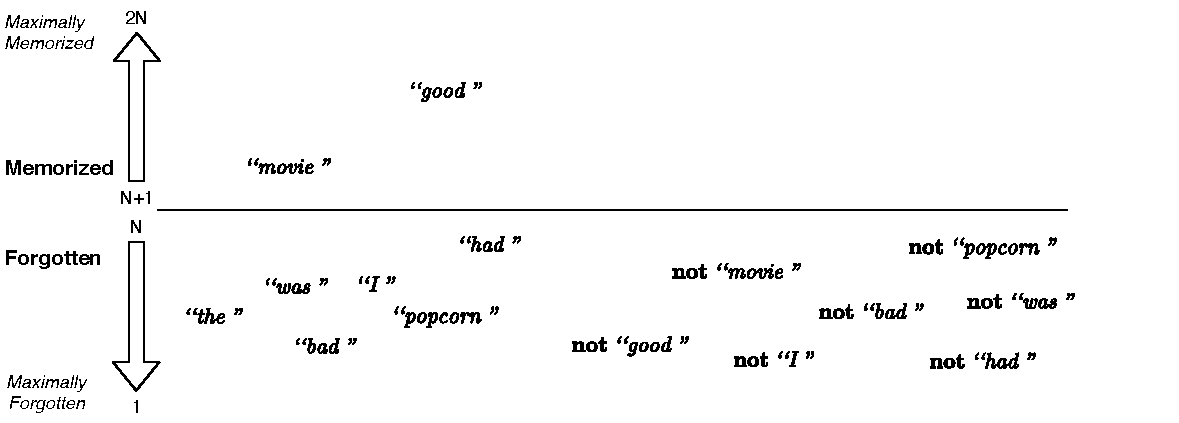
\includegraphics[width=.9\textwidth]{img/Memory_IMDb[2108.07594v1].pdf}
    \caption[Sticky memory for IMDb example]{Sticky memory for IMDb example with depth N for the clause: ``good'' AND ``movie'' (source: \cite{glimsdal2021coalescedmultioutputtsetlinmachines})}
    \label{fig:memoryimdb}
\end{figure}
\FloatBarrier

\paragraph{Memory updating}
Memory is updated on a specific input $X$ to the TM. A user-defined parameter $s$ controls how quickly truth values are forgotten. In result, increasing $s$ makes the patterns finer (more specific), while decreasing $s$ makes them coarser (more general). The process of updating the memory of each clause is handled by these three operators~\cite{glimsdal2021coalescedmultioutputtsetlinmachines}:
\begin{compactitem}
    \item The $\textbf{memorize}(X,s)$ operator handles \textbf{Type Ia feedback} (Figure \ref{fig:memoryimdbtypeIa}). It strengthens the memory of an input $X$ by increasing integer values for truth values present in $X$. Simultaneously, truth values that conflict with the input have their integers decreased randomly with probability $\frac{1}{s}$.
    \item The $\textbf{forget}(s)$ operator handles \textbf{Type Ib feedback} (Figure \ref{fig:memoryimdbtypeIb}). It performs forgetting by randomly decreasing the memory integer of all truth values with probability $\frac{1}{s}$. This gradually moves all literals towards the ``maximally forgotten'' state.
    \item The $\textbf{invalidate}(X)$ operator handles \textbf{Type II feedback} (Figure \ref{fig:memoryimdbtypeII}). It adjusts the clause to reject the input $X$ by increasing the memory integer of all False truth values. For instance, if the word ``bad'' appears in a negative review that was incorrectly classified, the system increases the integer for \textbf{not} ``bad''.
\end{compactitem}

\begin{figure}[!htbp]
    \centering
    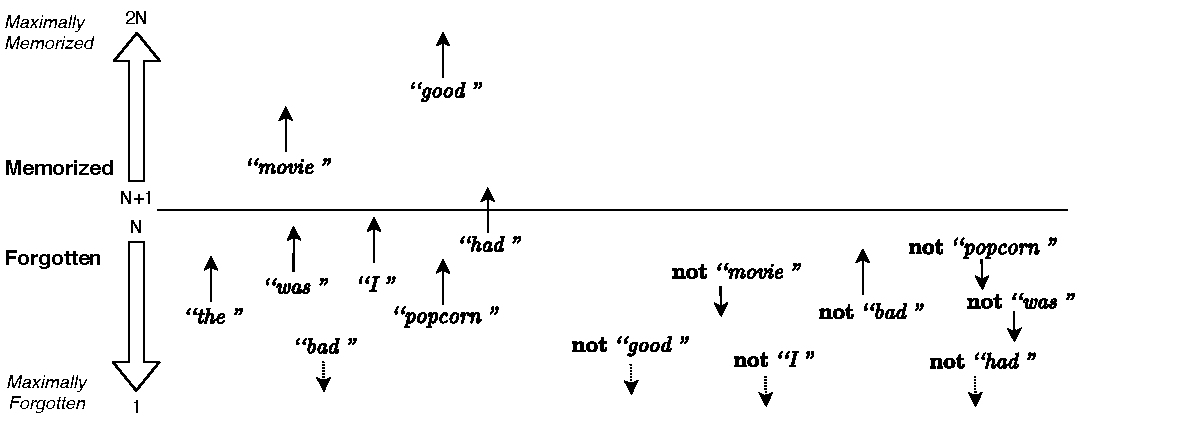
\includegraphics[width=.9\textwidth]{img/Memory_IMDb_Type_Ia[2108.07594v1].pdf}
    \caption[Type Ia feedback for IMDb example]{Type Ia feedback triggered by input ``The movie was good, and I had popcorn.'' (source: \cite{glimsdal2021coalescedmultioutputtsetlinmachines})}
    \label{fig:memoryimdbtypeIa}
\end{figure}
\FloatBarrier

\begin{figure}[!htbp]
    \centering
    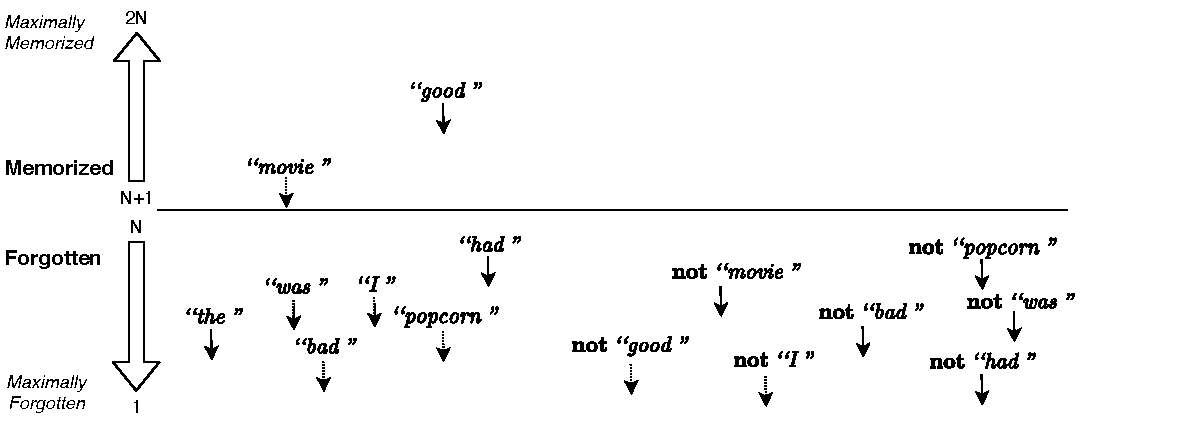
\includegraphics[width=.9\textwidth]{img/Memory_IMDb_Type_Ib[2108.07594v1].pdf}
    \caption[Type Ib feedback for IMDb example]{Type Ib feedback triggered by input ``Was good, and I had popcorn.'' (source: \cite{glimsdal2021coalescedmultioutputtsetlinmachines})}
    \label{fig:memoryimdbtypeIb}
\end{figure}
\FloatBarrier

\begin{figure}[!htbp]
    \centering
    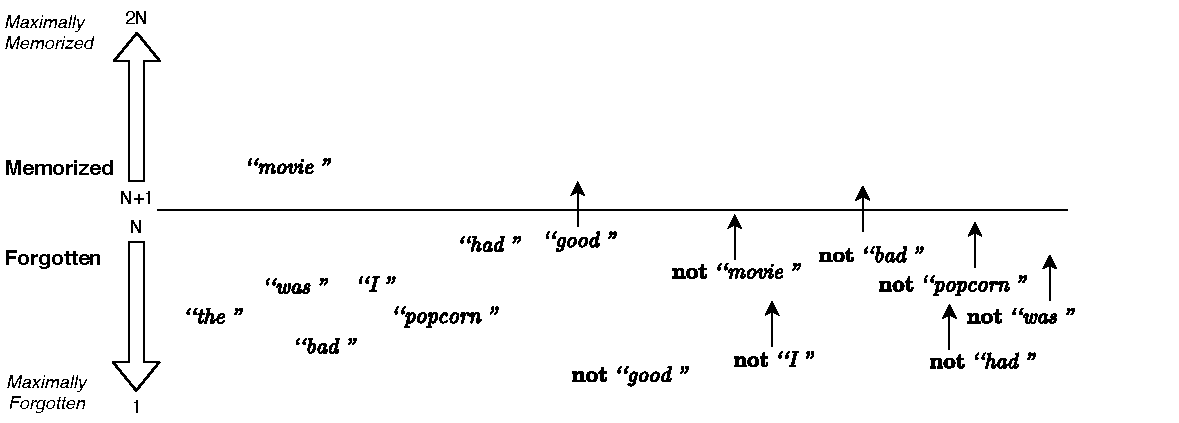
\includegraphics[width=.9\textwidth]{img/Memory_IMDb_Type_II[2108.07594v1].pdf}
    \caption[Type II feedback for IMDb example]{Type II feedback applied to input ``The movie was bad, and I had popcorn.'' (source: \cite{glimsdal2021coalescedmultioutputtsetlinmachines})}
    \label{fig:memoryimdbtypeII}
\end{figure}
\FloatBarrier

\paragraph{Learning single clauses}
Prediction outcomes guide the learning of each TM clause~\cite{glimsdal2021coalescedmultioutputtsetlinmachines}:
\begin{compactitem}
    \item \textbf{True Positive}: The clause correctly votes for its assigned output. In this case, the clause performs $\textbf{memorize}(X,s)$. This feedback makes the clause remember and refine the pattern it recognizes in $X$.
    \item \textbf{False Negative}: The clause fails to vote for its assigned output. In this case, the clause performs $\textbf{forget}(s)$. This reinforcement coarsens infrequent patterns, making them frequent.
    \item \textbf{False Positive}: The clause incorrectly votes for its assigned output. The clause then performs $\textbf{invalidate}(X)$. This feedback makes the clause more discriminative.
    \item \textbf{True Negative}: The clause correctly refrains from voting for its assigned output. This outcome does not trigger any memory updates.
\end{compactitem}

\paragraph{Learning multiple clauses}
The TM achieves coordination by introducing another parameter, a voting margin $t$. This ensures that a sufficient number of clauses support each output without using more clauses than necessary. Learning multiple clauses works as follows~\cite{glimsdal2021coalescedmultioutputtsetlinmachines}:
\begin{compactenum}
    \item \textbf{Input:} Consider a training sample of truth values $X$ and the target truth value $y$.
    \item \textbf{Vote Aggregation:} Compute the net voting sum $v$ by aggregating the output of all clauses that evaluate to \textit{True} on input $X$. Votes in favor of the target class $y$ are positive, while votes in favor of $\textbf{not } y$ are negative. The final sum $v$ is clipped to the range $[-t, t]$.
    \item \textbf{Stochastic Update:} A feedback update for each clause is triggered with probability $P_\text{update} = \frac{t-v}{2t}$. If triggered, the clause is modified as follows:
    \begin{compactenum}
        \item \textbf{True Positives (Type Ia feedback):} Perform $\textbf{memorize}(X,s)$ (the clause matches $X$ and outputs $y$)
        \item \textbf{False Negatives (Type Ib feedback):} Perform $\textbf{forget}(s)$ (the clause does not match $X$ and outputs $y$)
        \item \textbf{False Positive (Type II feedback):} Perform $\textbf{invalidate}(X)$ (the clause matches $X$ and outputs $\textbf{not } y$)
    \end{compactenum}
\end{compactenum}

\paragraph{XOR-gate example}
Figure \ref{fig:tsetlinmachinexorgate} illustrates the learning process for an XOR-gate training sample with input $(x_1=0,x_2=1)$ and target output $y=1$. Initially (Step $1$), the positive clauses $C_1$ and $C_3$ do not match the input because they contain conflicting literals (e.g. $\overline{x_2}$ in $C_3$ conflicts with $x_2=1$). This results in a false negative prediction,. which triggers Type Ib feedback. This feedback forces the clause to forget the conflicting literals. Once the clauses are generalized enough to match the input, Type Ia feedback reinforces inclusion of valid literals present in the input (e.g. $x_2$ in $C_3$). By Step $t$, these updates modified Clause $C_1$ to $\overline{x_1}x_2$ and $C_3$ to just $x_2$ allowing the machine to match the input and produce the correct prediction $\hat{y}=1$.

\begin{figure}[!htbp]
    \centering
    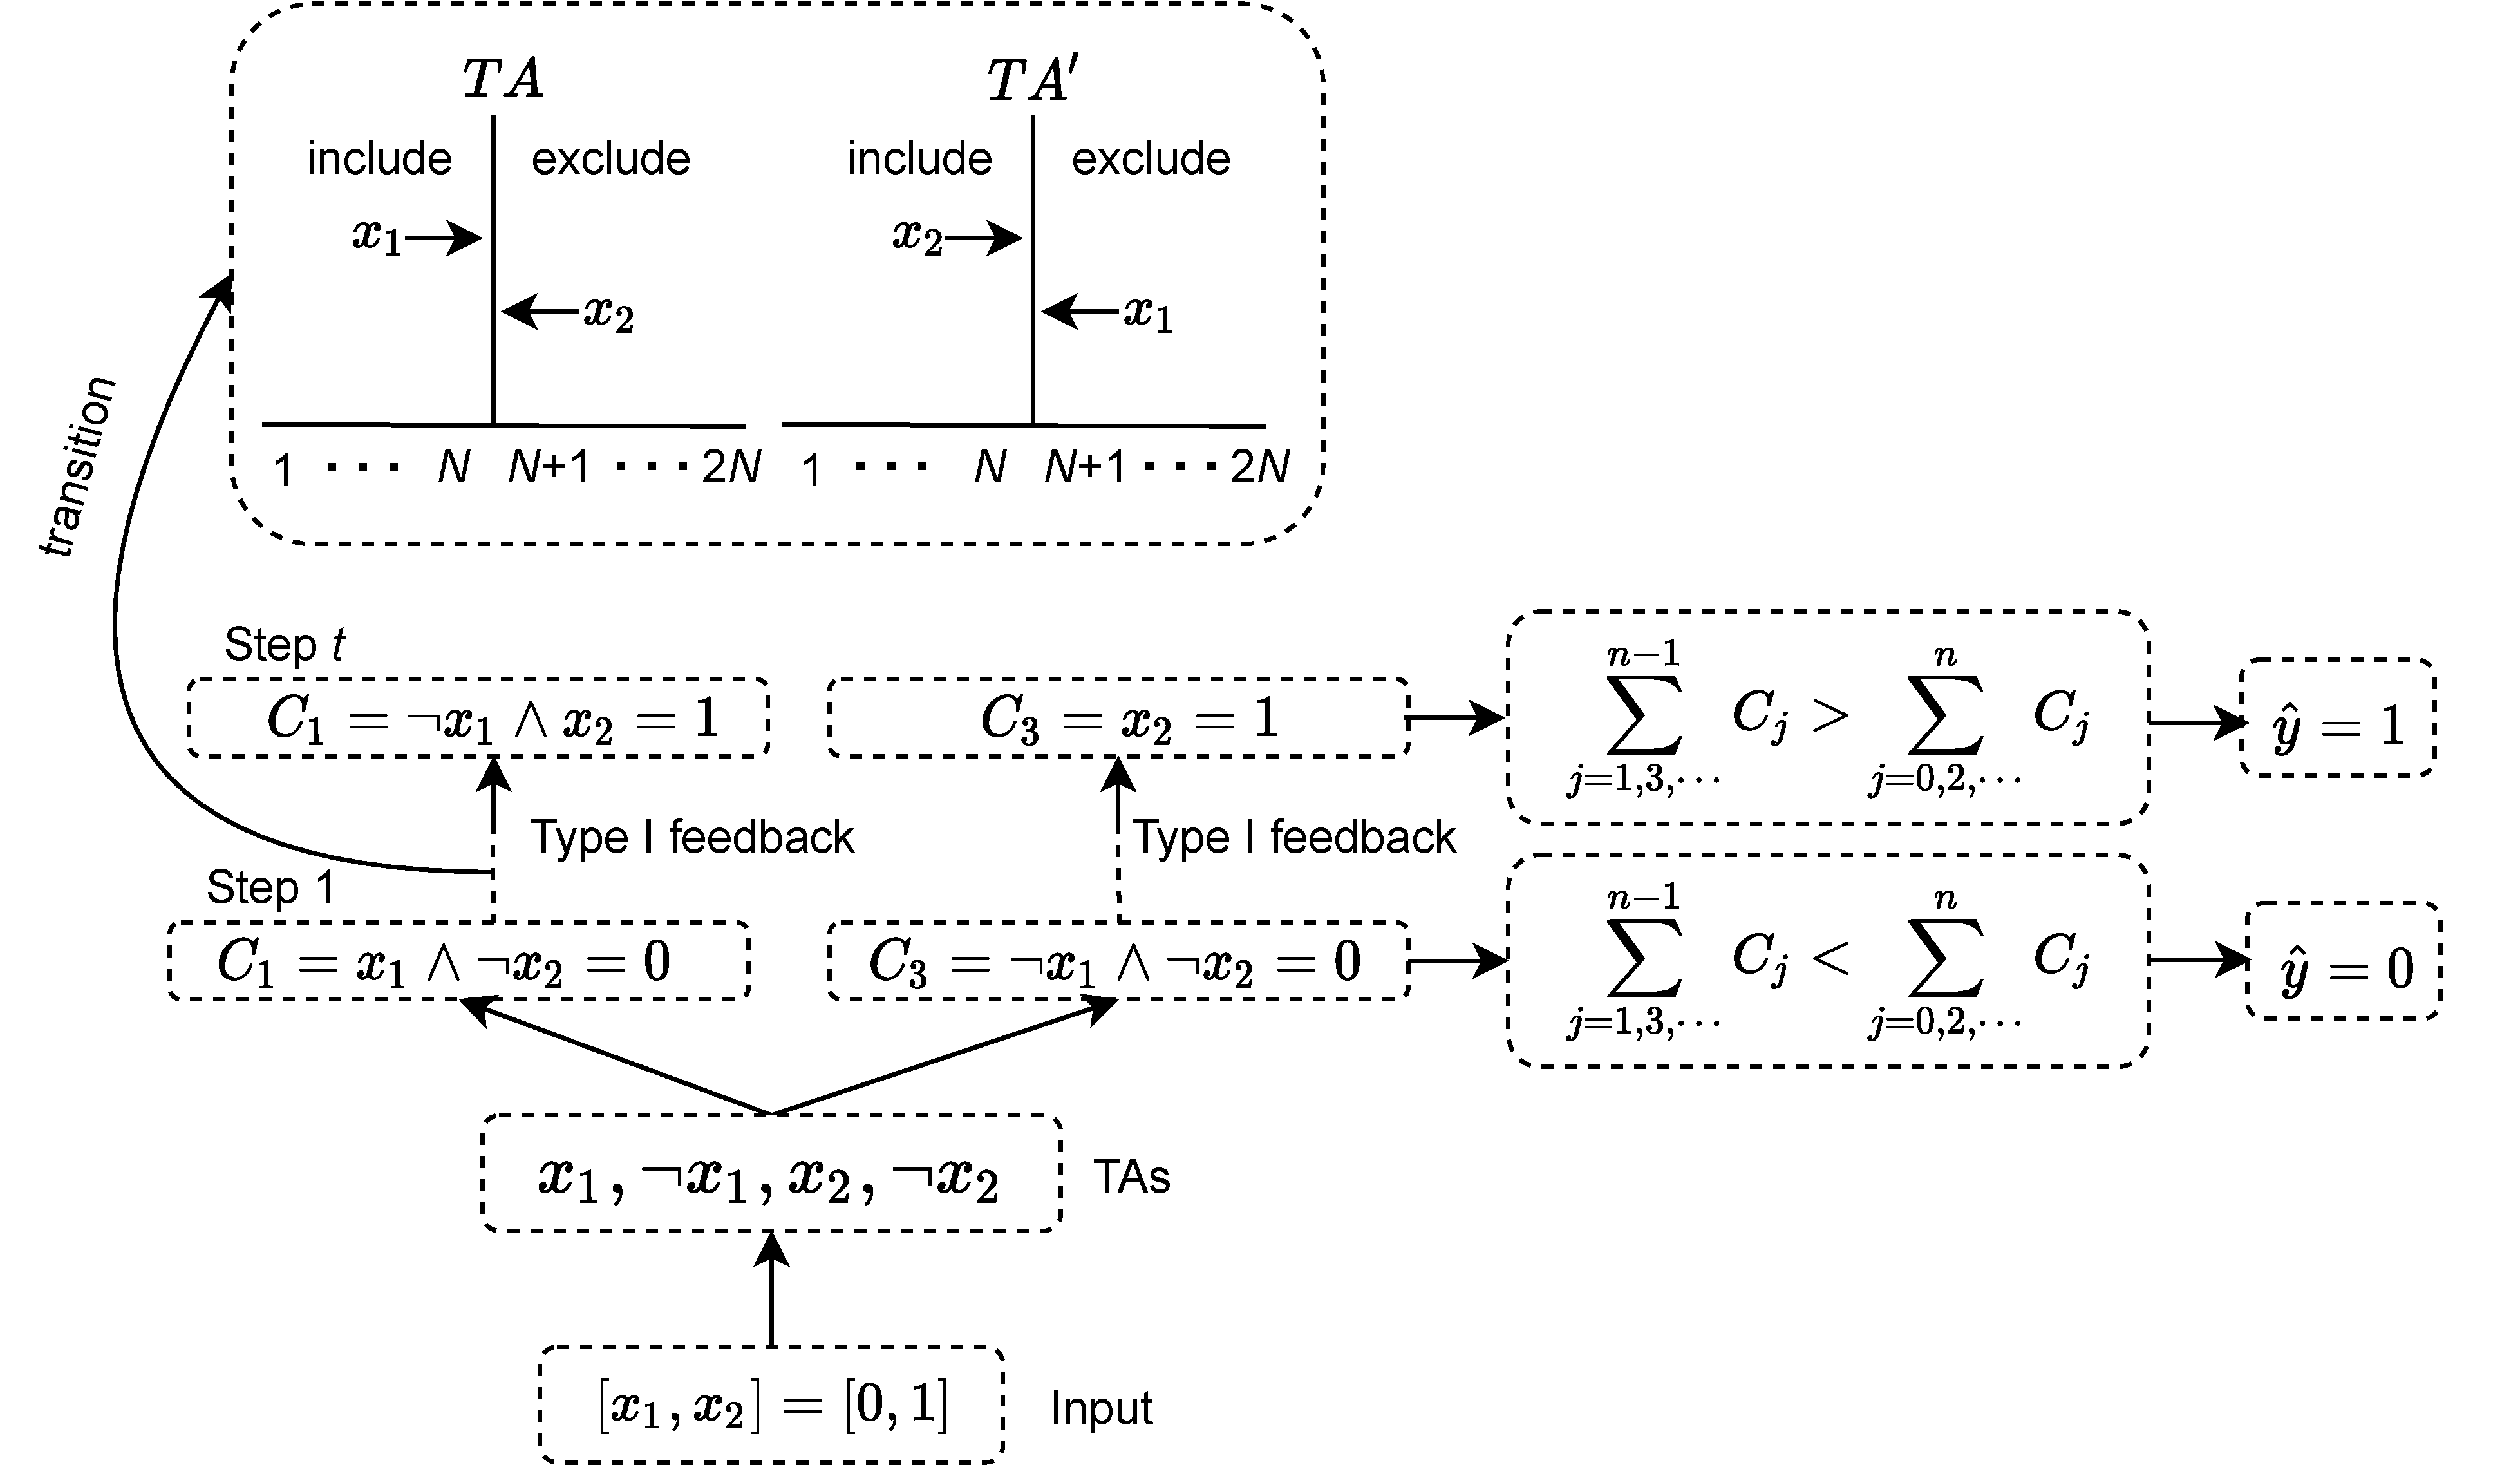
\includegraphics[width=.9\textwidth]{img/TM[arXiv-2212.13634v1].pdf}
    \caption[TM XOR-gate training]{TM learning dynamics for an XOR-gate training sample, with input $(x_1 = 0, x_2 = 1)$ and output target $y = 1$ (source: \cite{sharma2022equivalenceweightedtsetlinmachine})}
    \label{fig:tsetlinmachinexorgate}
\end{figure}
\FloatBarrier

\section{Tsetlin Machine Architecture Variants}
Due to the modular design of the original TM, there is an ongoing effort to further develop this method. Researchers have implemented new iterations to address and mitigate limitations discovered in the original design. In this section, we briefly discuss three significant architectural variations and what they attempt to accomplish.

\paragraph{The Coalesced Tsetlin Machine}\label{para:cotm}
The standard design of the TM supports prediction for only a single binary output. Multi-output problems require a workaround where a separate machine is created for every output. This approach in which each machine works independently limits the ability to share patterns that may be relevant to multiple classes. The Coalesced TM~\cite{glimsdal2021coalescedmultioutputtsetlinmachines} introduces a shared pool of clauses. This is accomplished by a weight matrix that connects every clause to every possible output. Instead of a rule belonging to just one class, it is assigned an integer weight: a positive weight votes in favor of a class, while a negative weight votes against it. Empirical results on benchmark datasets show that this approach obtains significantly higher accuracy in 50 to 1000-clause configurations, indicating an ability to reuse clauses and stronger robustness against imbalanced training data~\cite{glimsdal2021coalescedmultioutputtsetlinmachines}. Figure \ref{fig:tsetlinmachinecoalesced} shows an inference structure with three outputs, a newly introduced clause memory matrix and a clause weight matrix.

\begin{figure}[!htbp]
    \centering
    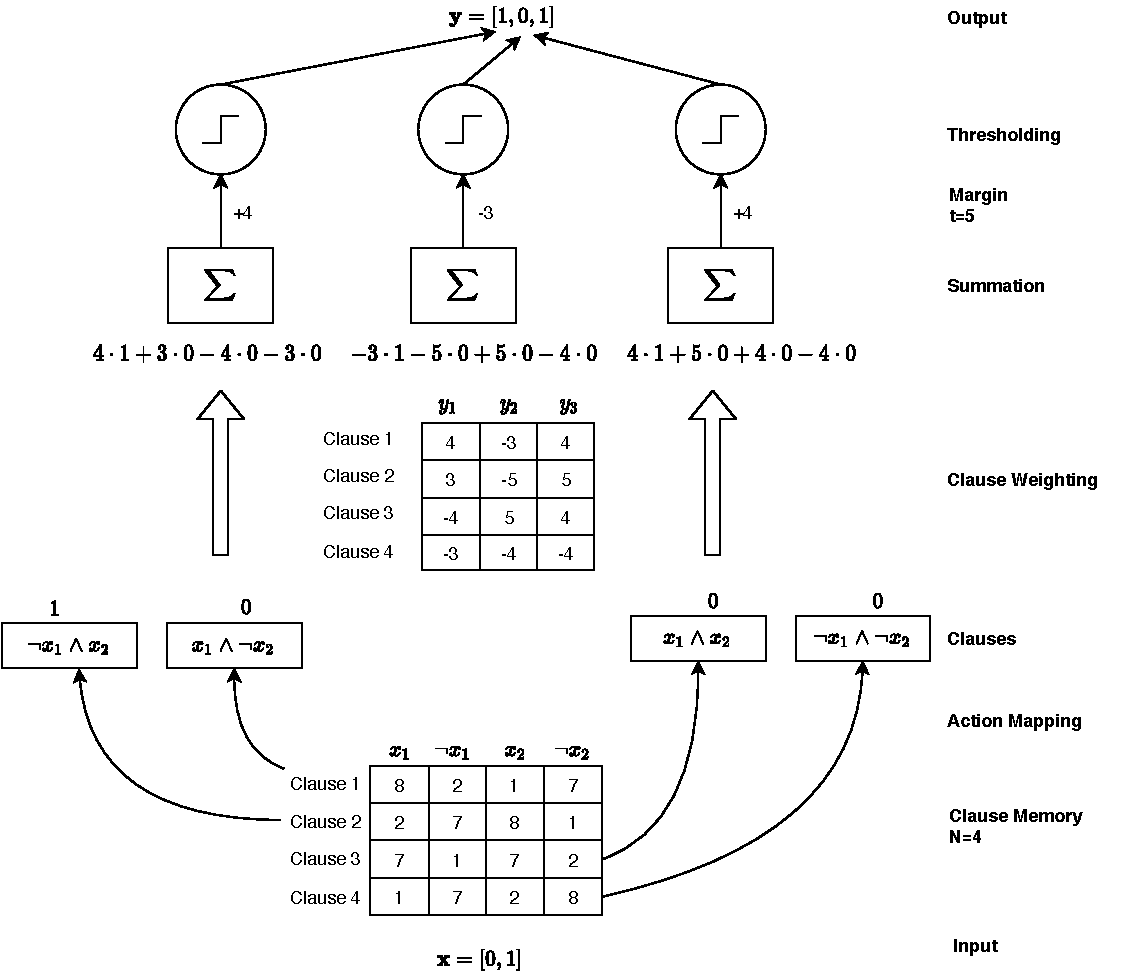
\includegraphics[width=.9\textwidth]{img/CoalescedMultiOutputTM[2108.07594v1].pdf}
    \caption[The Coalesced TM structure]{The Coalesced TM structure with inference example (source: \cite{glimsdal2021coalescedmultioutputtsetlinmachines})}
    \label{fig:tsetlinmachinecoalesced}
\end{figure}
\FloatBarrier

\paragraph{The Sparse Tsetlin Machine}
The standard TM maintains the entire state space, storing a significant number of unnecessary values that consume memory and computational time. The Sparse TM~\cite{glimsdal2024sparsetsetlinmachine} addresses this by implementing the \textit{Active Literals} mechanism, which focuses resources only on actively contributing literals. To achieve this, the architecture utilizes the Compressed Sparse Row (CSR) format and discards negated features, assuming that any missing feature is implicitly negated. A lower-bound threshold is added to ensure the compactness of the model, where any literal state reduced below the limit is removed from the clause. This significantly reduces memory footprint and computational time while maintaining competitive classification performance~\cite{glimsdal2024sparsetsetlinmachine}. Figure \ref{fig:tsetlinmachinesparse} illustrates the feedback interaction between \textit{Active Literals} and sparse clauses. During Type Ia feedback (reinforcing true positives), \textit{Active Literals} identify and store meaningful literals, while Type II feedback (combating false positives) introduces these literals into the sparse clauses to invalidate incorrect matches.

\begin{figure}[!htbp]
    \centering
    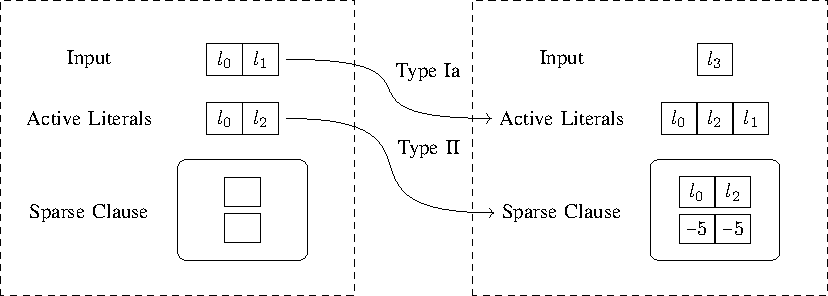
\includegraphics[width=.9\textwidth]{img/sparse_al_populate[arXiv-2405.02375v2].pdf}
    \caption[The Sparse TM Active Literals]{The Sparse TM using Active Literals (source: \cite{glimsdal2024sparsetsetlinmachine})}
    \label{fig:tsetlinmachinesparse}
\end{figure}
\FloatBarrier

\paragraph{The Stateless (Inference Only) Tsetlin Machine}
There is a major difference between how the TM learns and how it makes predictions. During the learning phase, the machine relies on a detailed memory state to track pattern confidence, storing a state integer (ranging from $1$ to $2N$) for every potential literal. However, once training is completed, this detailed history is no longer needed to make predictions. For inference, the model only needs to know which specific literals to Include and which to Exclude, converting complex memory states into simple binary rules. By discarding learning memory and keeping only the final compiled rules, the model significantly reduces memory usage during deployment when on-device learning is not required. For example, in Figure \ref{fig:memoryimdb}, the inference model would discard the forgotten values and store only the final rule: ``good'' AND ``movie''.

\section{Comparison with Neural Networks}
Neural Networks are currently the standard approach for AI applications, making them the common benchmark for new methods. For a direct theoretical comparison, the research conducted in~\cite{sharma2022equivalenceweightedtsetlinmachine} introduced the Weighted TM. This architecture assigns an integer weight to each clause based on its prediction accuracy, operating similarly to the Coalesced TM (Section \ref{para:cotm}) but without the clause sharing mechanism. With this modification, the TM behaves as a special case of a perceptron using logical clauses as binary inputs instead of raw features~\cite{sharma2022equivalenceweightedtsetlinmachine}.

The difference in the decision boundaries on the Iris dataset is illustrated in Figure \ref{fig:decisionboundaryvis}, where each model was trained for $50$ epochs. The TM (Figure \ref{fig:tsetlinmachinevis}) used 50 clauses and the Single Layer Neural Network (Figure \ref{fig:neuralnetworkvis}) utilized 50 neurons. The TM builds its decision boundaries from the binary output of individual clauses ($C_i = \{0, 1\}$). It results in steps formed by filling contour lines rather than the smooth curves generated by neural networks. This difference changes how each model adapts to new data. In the TM, a clause (or a set of clauses) can simply learn the new pattern and create a step in the decision boundary to include the new data point in the correct region~\cite{sharma2022equivalenceweightedtsetlinmachine}.

\begin{figure}[!htbp]
    \centering
    % Subfigure 1
    \begin{subfigure}{0.3\textwidth}
        \centering
        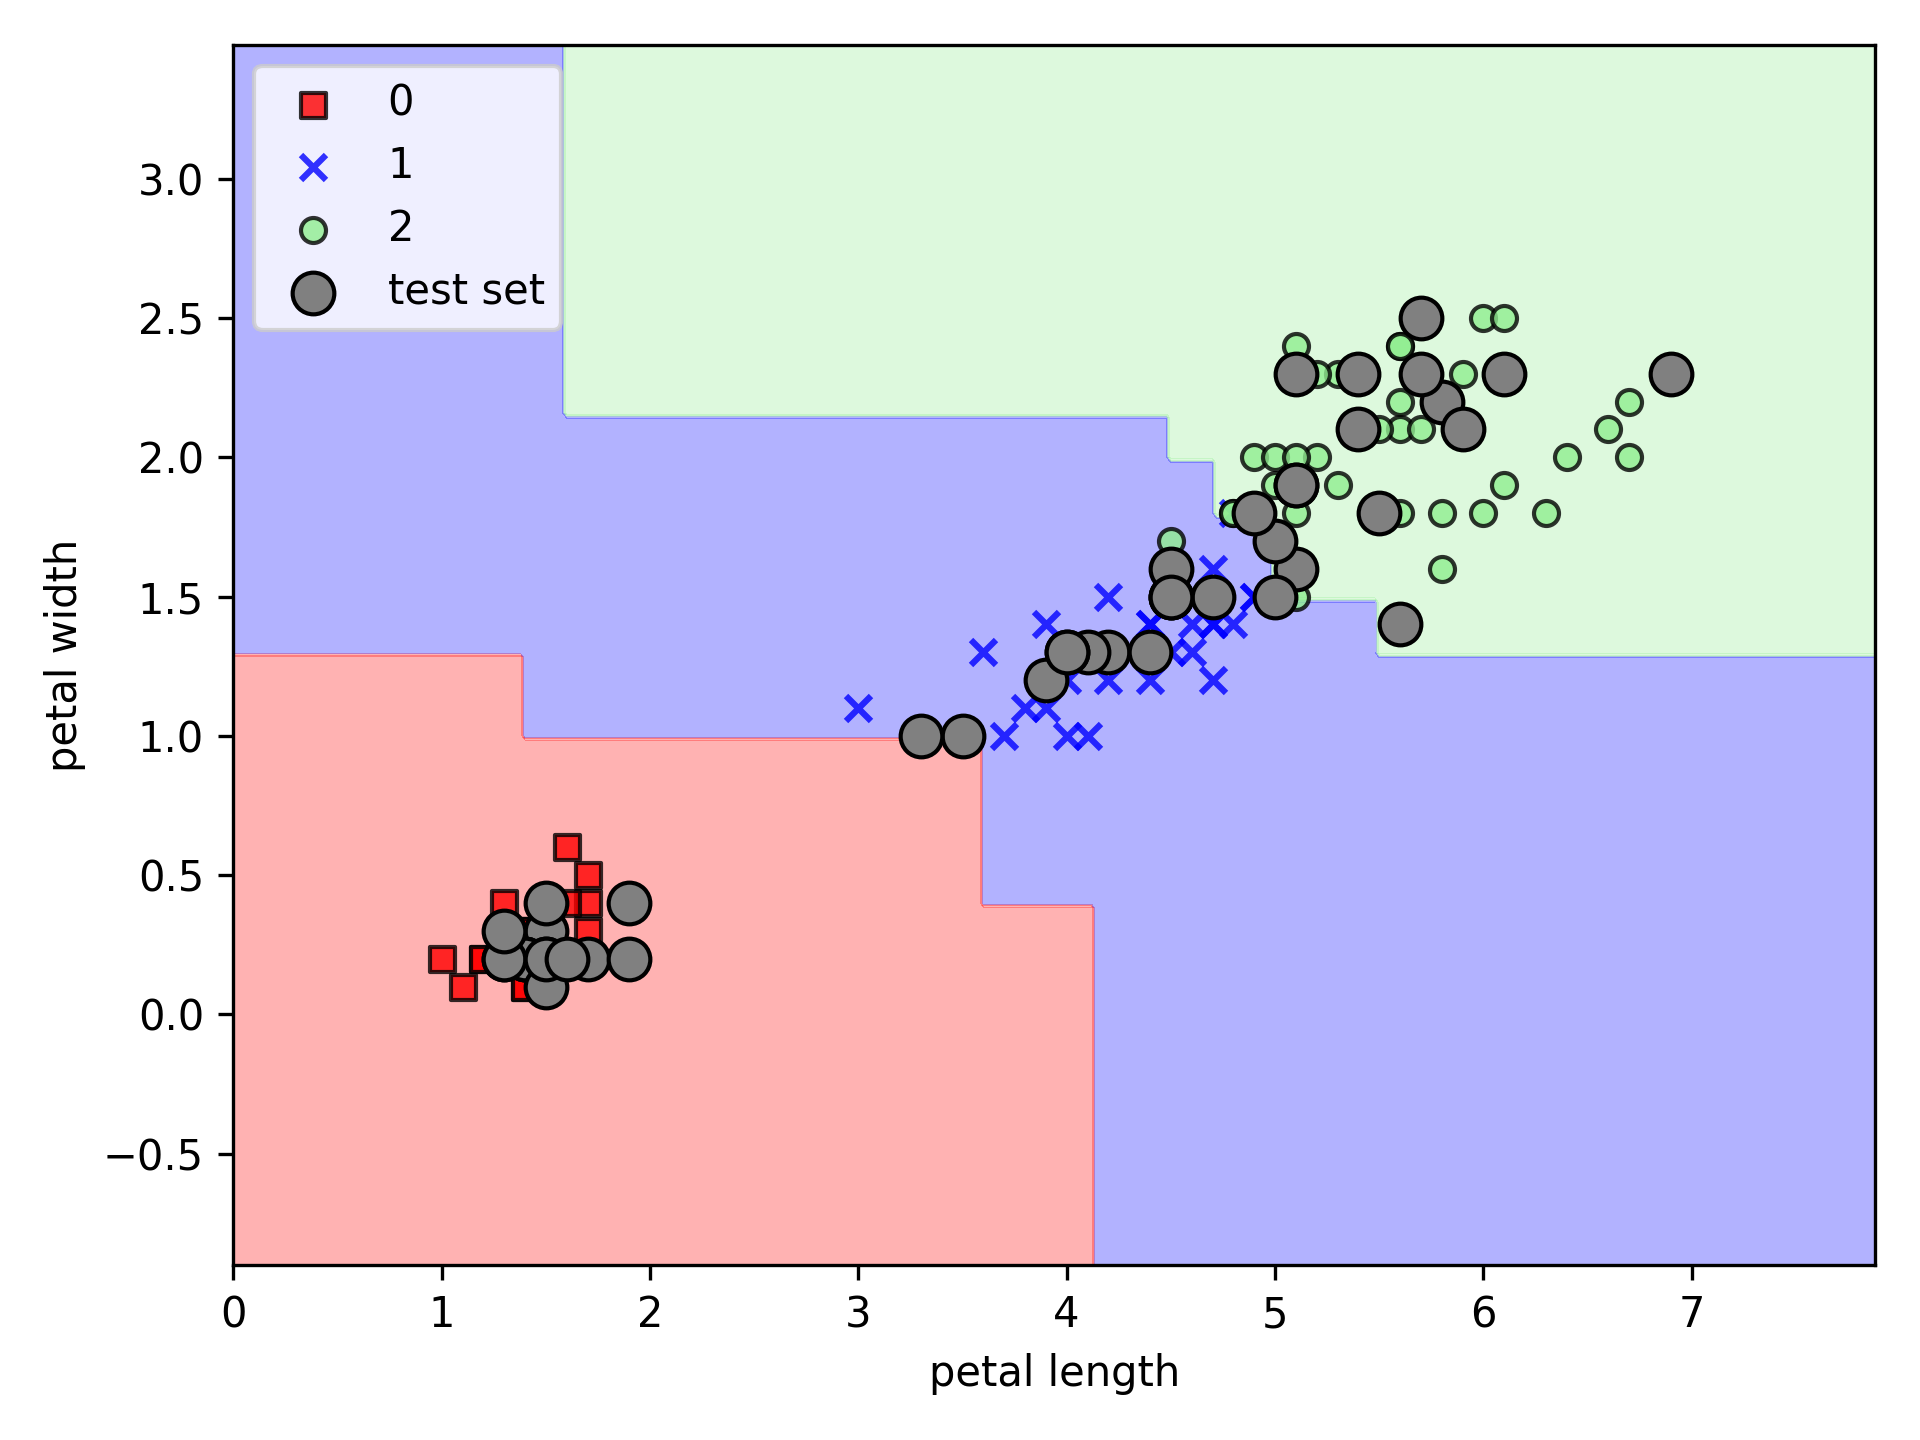
\includegraphics[width=\textwidth]{img/tm_vis[arXiv-2212.13634v1].png}
        \caption{TM}
        \label{fig:tsetlinmachinevis}
    \end{subfigure}
    \hfill
    % Subfigure 2
    \begin{subfigure}{0.3\textwidth}
        \centering
        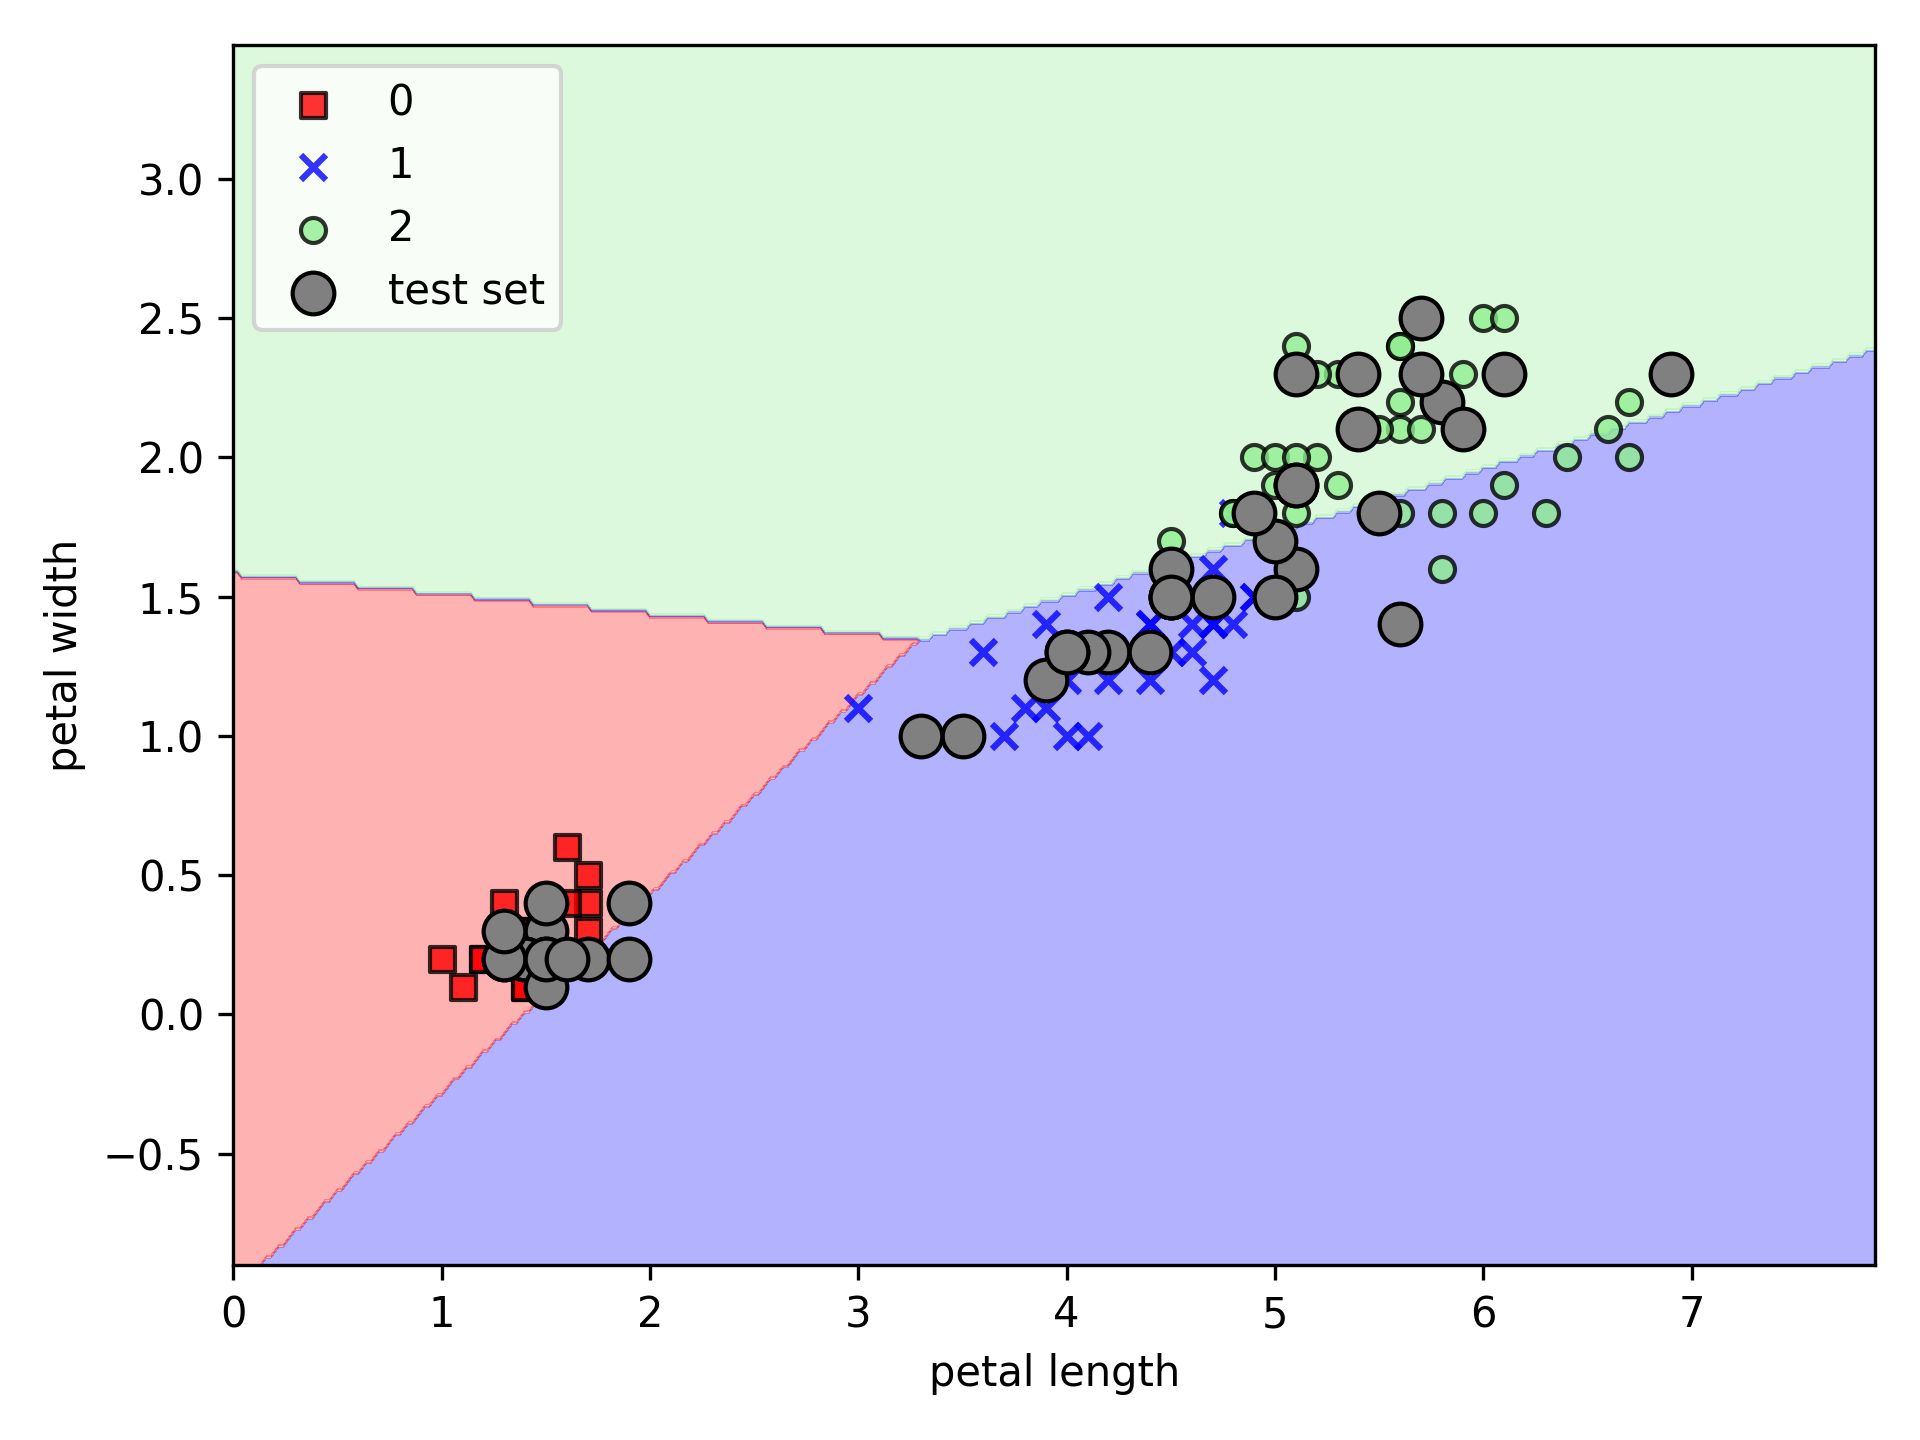
\includegraphics[width=\textwidth]{img/perceptron_vis[arXiv-2212.13634v1].png}
        \caption{Perceptron}
        \label{fig:perceptronvis}
    \end{subfigure}
    \hfill
    % Subfigure 3
    \begin{subfigure}{0.3\textwidth}
        \centering
        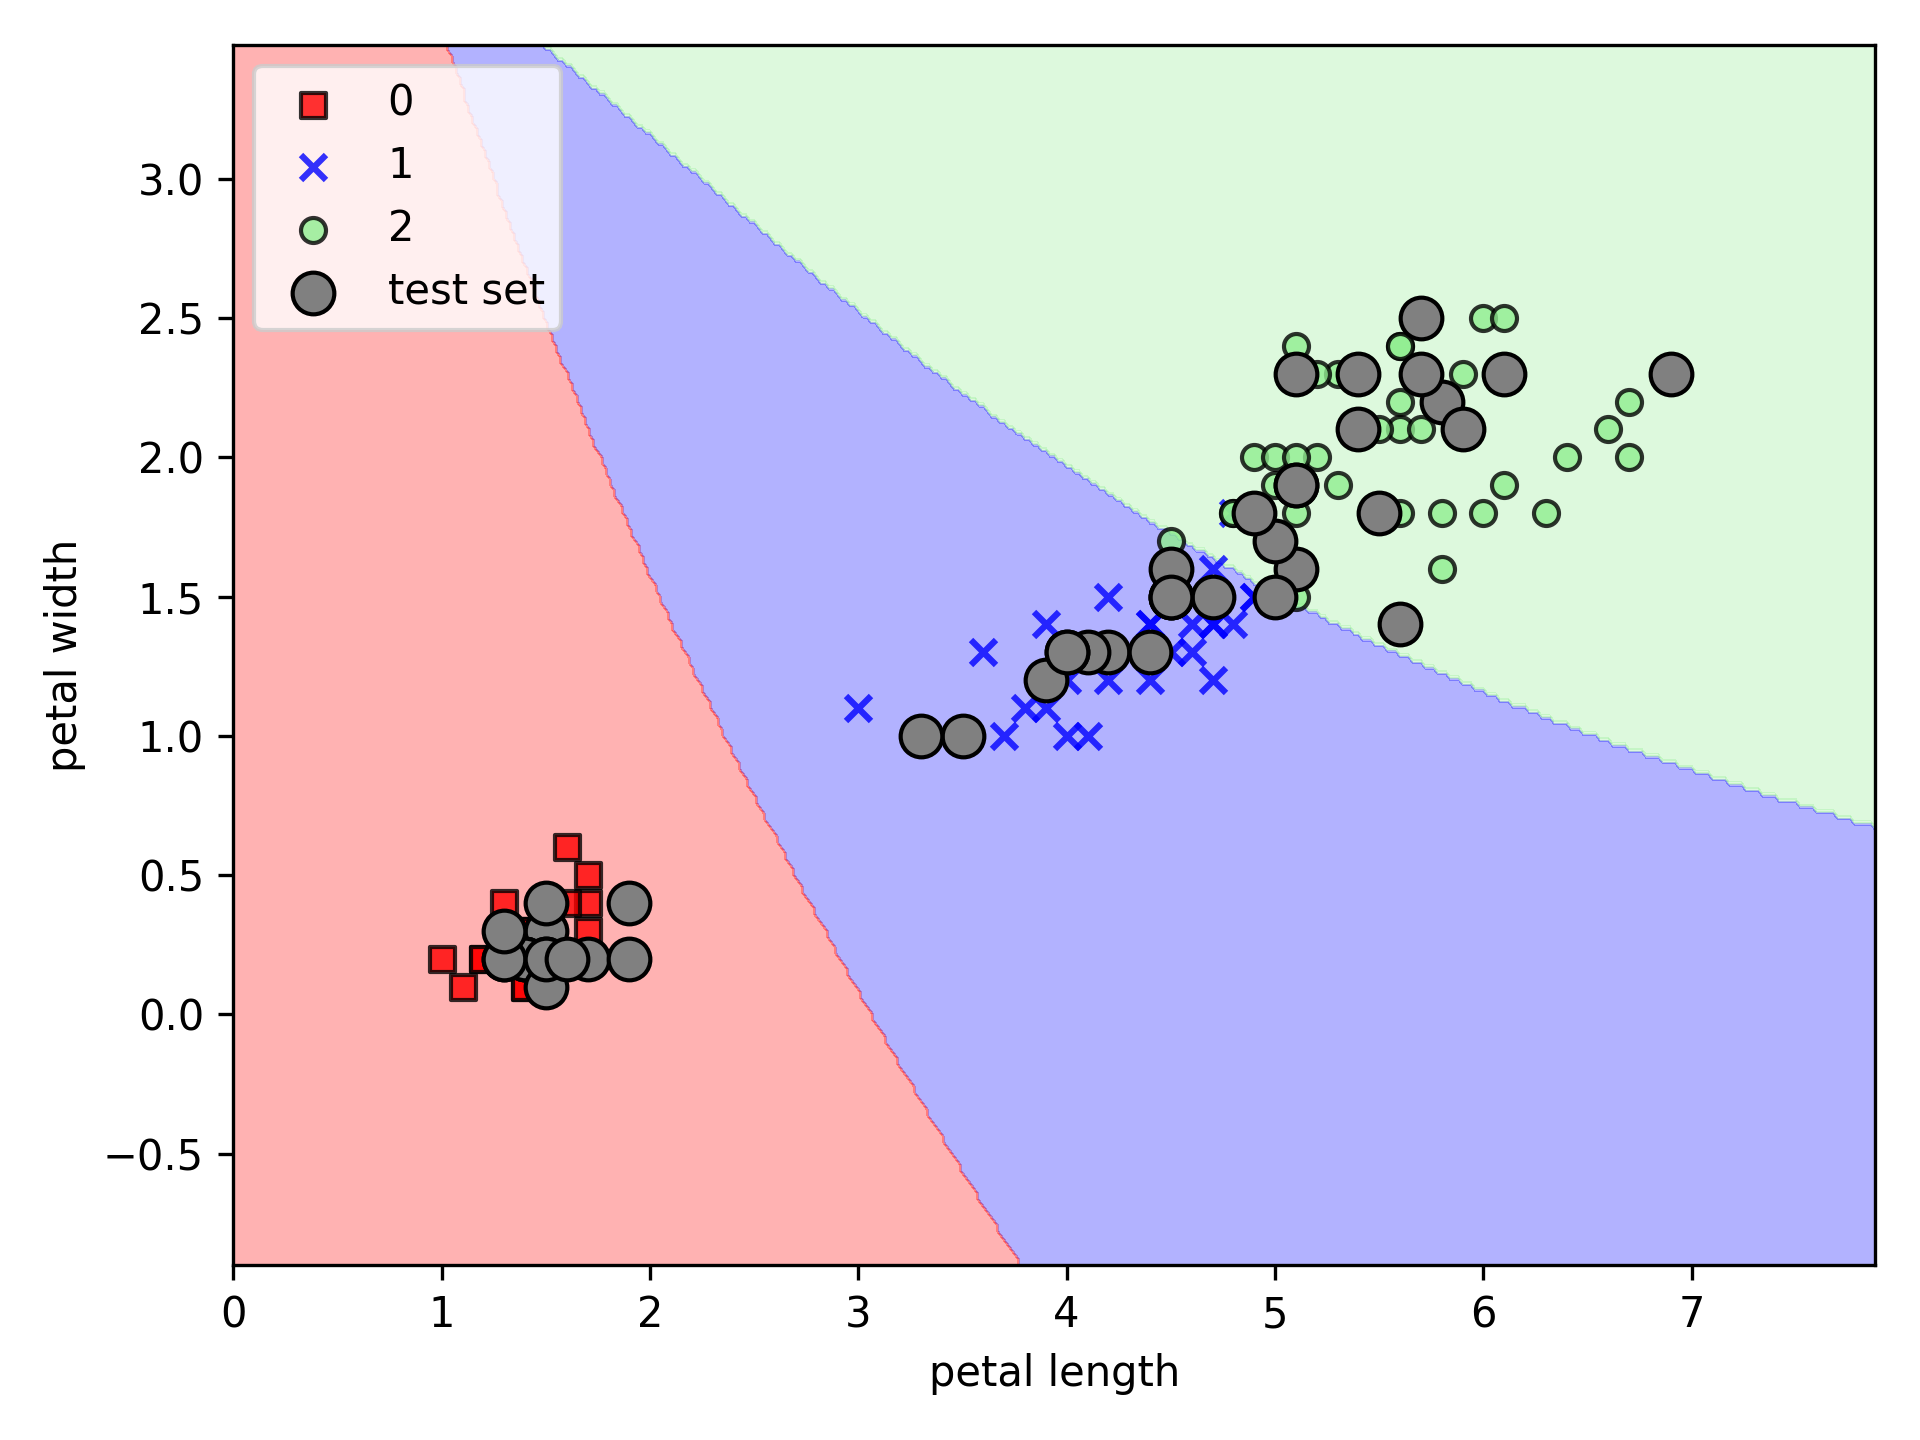
\includegraphics[width=\textwidth]{img/mlp_vis[arXiv-2212.13634v1].png}
        \caption{Single Layer NN}
        \label{fig:neuralnetworkvis}
    \end{subfigure}

    \caption[Decision boundary visualization]{Decision boundary visualization on the Iris dataset (source: \cite{sharma2022equivalenceweightedtsetlinmachine})}
    \label{fig:decisionboundaryvis}
\end{figure}
\FloatBarrier

\paragraph{Transparent logic}
Neural networks are often described as ``black boxes'' because their decision making logic is hidden and difficult for humans to interpret. This contrasts with the TM, where interpretability comes naturally from its logic-based approach. The produced rules are human-readable clauses (e.g. \textit{if X and Y then Class A}), making it technically possible to even manually add or edit rules. This transparency allows users to examine the inner workings in applications where understanding the reasoning behind a prediction is mandatory.

\paragraph{Computational efficiency and optimization}
An important difference between the architectures lies in their underlying arithmetic. Neural networks typically rely on floating-point matrix multiplications that require substantial computational resources. In contrast, the TM operates primarily using bitwise operators (AND, OR, NOT) and simple integer arithmetic. Theoretically, this offers efficiency advantages, enabling implementations on hardware lacking dedicated floating-point units. However, modern processors such as GPUs and TPUs are specifically engineered to accelerate matrix operations, since they are widespread in fields ranging from physics simulations to deep learning. As a result, the performance advantage of an integer-based approach is diminished on hardware that implements these optimizations.

\paragraph{Performance with limited data}
According to research presented in~\cite{granmo2021tsetlinmachinegame}, TMs generalize better with smaller datasets compared to neural networks. In benchmarks such as the Noisy XOR problem, the TM maintained much higher accuracy on smaller datasets, whereas neural networks required larger datasets to converge. This makes the TM a suitable candidate for environments where data is limited or noisy.

\section{Summary}
In conclusion, the Tsetlin Machine is a logic-based alternative for pattern recognition that utilizes Boolean algebra. It is built upon Tsetlin Automata, which are finite-state machines that learn optimal actions through rewards and penalties. These automata are arranged into teams to construct ``If-Then'' rules known as conjunctive clauses, which identify sub-patterns in data. Then these clauses are for or against a target class to reach a final decision. The model is trained using a game-theoretic algorithm that employs different types of feedback to memorize, forget, or invalidate patterns. Compared to traditional ``black box'' neural networks, the Tsetlin Machine benefits from transparent logic and efficiency, both with computational resources and training data. Finally, recent architectural variants such as Coalesced, Sparse, and Stateless Tsetlin Machines address limitations of the original design.